%---------------------------------------------------------------------------------------------------
%		use-cases.tex
%
%	This file contains the sections that describe typical use cases on which we can find the problem
% that will be studied in the master thesis.
%
%	Author: Andrea Meneghinello
% Version: 0.1
%	Table of changes:
%		06/03/2016 -> document definition
%---------------------------------------------------------------------------------------------------
\section{Problem definition}
\label{sec:background-problem}
Nowadays more and more business companies use complex software systems in their daily activities;
from the customer care to internal administration. Until recently, these complex applications are
executed over proprietary hardware systems. This scenario is unfavourable for both companies and
software-houses that have to maintain the applications.

From the companies point of view, in order to keep those applications working, according
to the defined \glossarySng{sla}, they have to invest economic resources in qualified personnel and 
establish complex administration processes. They can solve this problem through the adoption of 
one of the many existent frameworks that allows \acs{it} process management. A well known one is
\keyword{\ac{itil}}. The framework, shown in Figure \ref{img:background-problem-itilProcessModel}, 
defines general best-practices in order to design and instantiate processes that permit a more coherent
administration of \acs{it} departments and the deployed applications. The processes that are relevant
for this problem belong to \ac{sda}. They are  \keyword{\ac{am}} and \keyword{\ac{cm}}. Both processes
focuses on planning and monitoring the effective provision of resources to support all the service
requirements \cite{availabilityCapacityProcesses}.

\begin{figure}
	\centering{}
	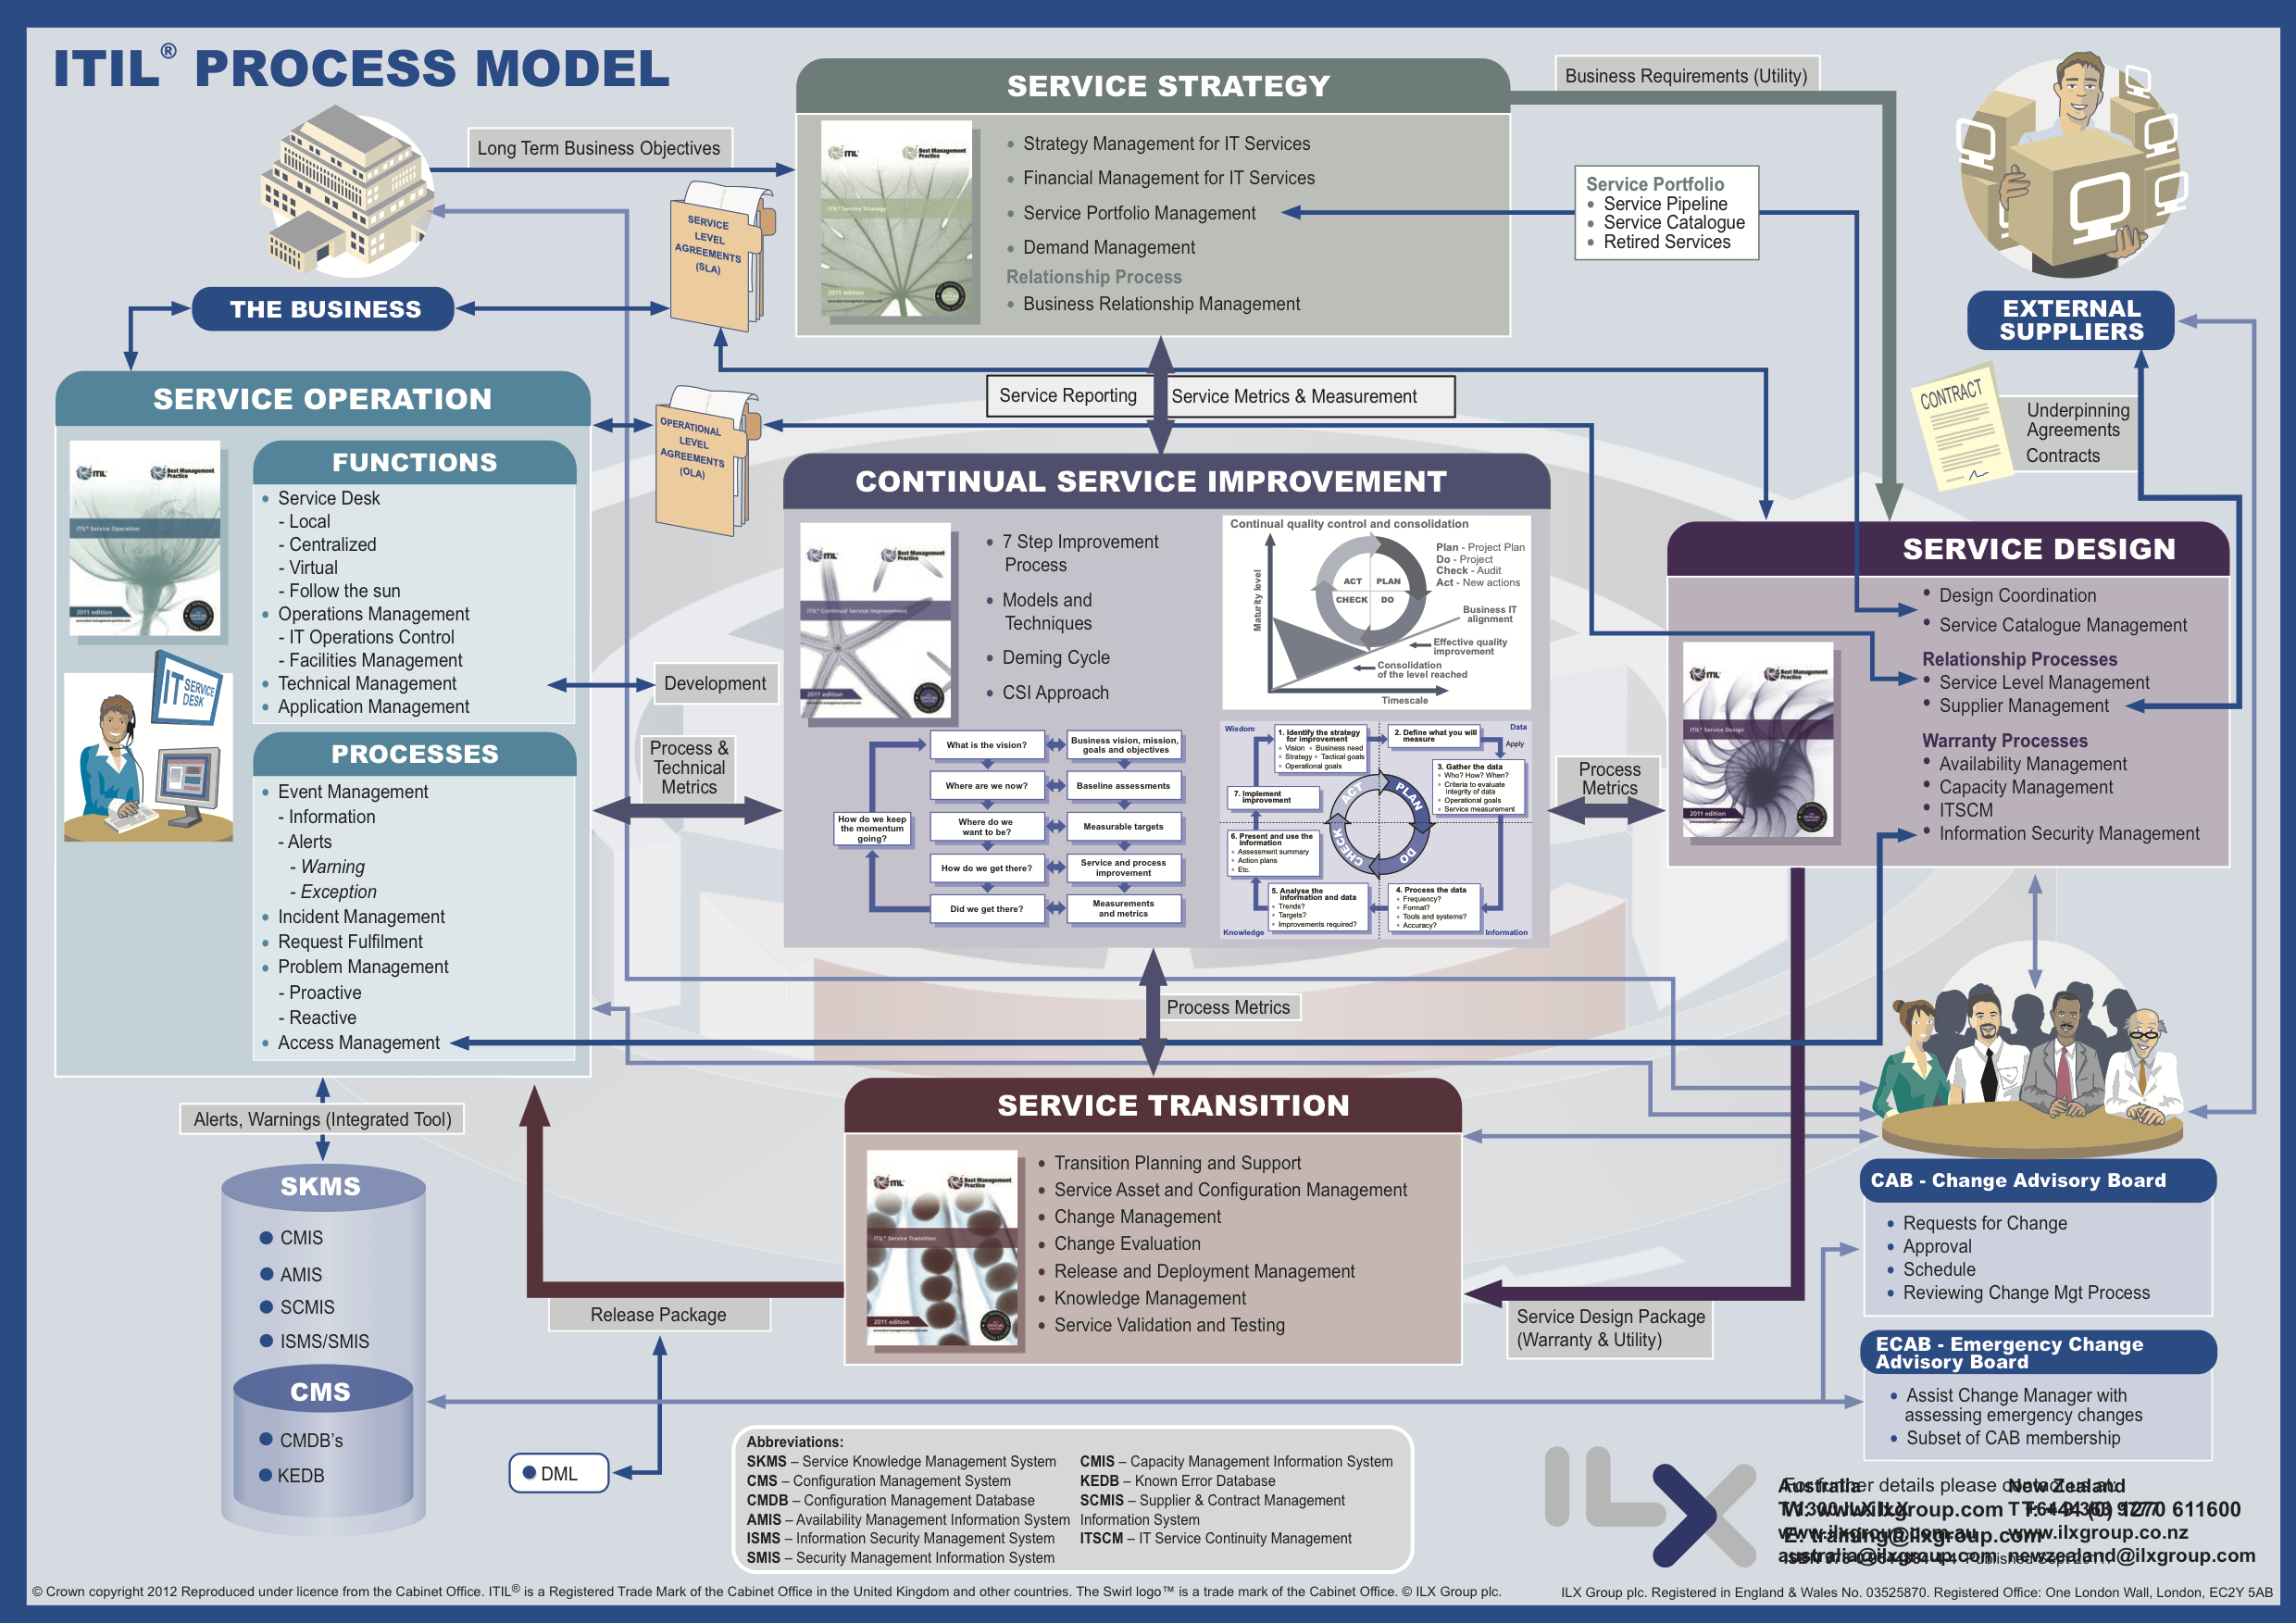
\includegraphics[width=0.8\textwidth]{chapters/background/images/itil-map.png}
	\caption[\acs{itil} v3 process model]{A bird's eye view of the processes defined by the \acf{itil} 
		framework. Their main purpose is to manage software's life-cycle in large business companies
		\cite{itilProcessModel}.}
	\label{img:background-problem-itilProcessModel}
\end{figure}

On the other hand software-houses have to face with different runtime environments (both in term of
hardware and software configurations) which makes the \glossaryPlr{deployment-process} more difficult.
Another problem is represented by unavoidable bug errors that are present in every application. Here
bugs are not only due to development errors but they can be also due to the runtime environment itself.
Thus developers waste a lot of time only to replicate those execution environments, stealing it from
more profitable activities. Finally when the solution is found they have to visit the client to fix
the bugs in loco (if remote assistance is not possible).

Another scenario is the following: software-houses may want to make their software available online
and always up-to-date. End-users should be able to use it anywhere and using any type of device without
any installation process. In addiction they do not have to care about updating that software.

Companies can follow general best-practices to solve the problem. In addiction, many of them have
understood, very well, the benefit of delegating hardware management to cloud providers (see Section
\ref{sec:background-cloudComputing-capexOpex}). Unfortunately, we cannot assert the same things for
software-houses.

Cloud computing is becoming more mature day by day and market has started investing on it. A recent
study, commissioned by Microsoft \cite{microsftCloudNewJob}, shows that cloud computing produces much
new innovation in \acs{it} every year:

\begin{center}
	\begin{quote}
		``Innovation created by cloud computing produce \textdollar{}1.1 trillion a year in new
		business revenues. It was also able to generate 14 million of jobs worldwide from 2011 to 2015.''
	\end{quote}
\end{center}

Therefore, the trend is positive and it is expected to grow more and more in the long term.
Lately, cloud computing model have become a more reliable infrastructure supplier, so companies 
started to earn outsourcing the hardware management. Nevertheless software engineers have to face
again with the construction and the configuration of complex scalable environments, stealing time from
development activities. As a consequence they ask for more automation in building work environments so
they can focus more on development activities (development, test and execution).

We have argued about the major requests made by software developers. Their need for automatic
hardware configuration and ready-to-use work environments promoted the creation of the \ac{paas} 
cloud model. \ac{paas} is one of the three conceptual layers in the \ac{spi} model: \ac{saas} on the
top (faces with end-users); \ac{paas} in the middle (faces with developers) and finally \ac{iaas} on
the bottom where physical resources reside (faces with sysadmins). The \ac{paas} layer is a good place
where managing the elasticity challenges and the related complexity.

%It differs from \ac{iaas} because \ac{paas} does not allow users to control the underlying
%hardware directly. In addiction, it also differs from the \ac{saas} layer because the latter is focused
%on software functionalities while the former is responsible on how the software is deployed and in managing
%the elasticity challenges and the related complexity. 

Despite all \ac{paas} advantages (described in Section \ref{sec:background-paas-characteristics})
the following issues may be still present:

\begin{itemize}
	\item{it may lead to a possible vendor lock-in if the provider imposes the use of a particular
		technology;}
	\item{it may compromise cloud resource elasticity because users are not able to configure the
		underlying hardware resources.}
\end{itemize}

In order for the \ac{paas} vendors to offer high quality services, both for companies and software-houses,
they must provide ready-to-use work environments and key mechanisms that guarantee \keyword{elasticity}
for the deployment units.

Elasticity is one of the key characteristics of the cloud and means that the cloud service can rapidly
scale its dimension according to the clients needs. It can be obtained by the combination of two complementary
dimensions: \keyword{optimization of the \ac{paas} underlying hardware management} and \keyword{specifically
designed software architectures}.

The assets on which the \ac{paas} vendors can make optimizations are those illustrated in Section
\ref{sec:background-virtualization-assets}, hence our contribution is to compare, and then analyse, the
infrastructural costs of both \ac{vm} and Docker based \ac{paas} solutions in terms of computing, storage and
networking. These assets allow \ac{paas} vendors to satisfy the elasticity requirements as better as they can.

In addiction we will seek for an architectural pattern that is able to exploit the elasticity mechanisms 
provided by the \ac{paas} layer.

Nowadays cloud computing is able not only to offer unlimited provision of hardware but also the generation
of dynamic work environments. In order to understand how it is possible we must first know what really is
cloud computing and why it is able to help both business companies and software-houses.